\documentclass[final,a0paper]{beamer}
%\documentclass[final,a1paper]{beamer}
\mode<presentation>{\usetheme{I6dv}}

\usepackage[orientation=landscape,size=a1,scale=1.8]{beamerposter}
\usepackage{exscale}
\usepackage{booktabs, array}
\usepackage[english]{babel}
\usepackage[latin1]{inputenc}
\usepackage{graphicx,color}
\usepackage{amsmath,amsthm,amssymb}
\usepackage{mpemath}
% \usepackage{algorithm}
% \usepackage{algorithmic}

\usepackage{linegoal}
\usepackage{mathtools}
\usepackage{color}
\usepackage{bm}
\usepackage[ruled,vlined,linesnumbered]{algorithm2e} %linesnumbered
\usepackage{etoolbox}

% \usepackage{algorithm}
% \usepackage{algorithmic}
%\usepackage{algpseudocode}

 \usepackage{tikz}
% \usetikzlibrary{arrows,automata}
\usepackage{graphicx}
\usetikzlibrary{arrows,decorations.markings}

\usepackage{pifont}% http://ctan.org/pkg/pifont
\newcommand{\cmark}{\ding{51}}%
\newcommand{\xmark}{\ding{55}}%

\renewcommand{\ss}{\mid}
\newcommand{\rtp}{\mathcal{P}} 
\newcommand{\rob}{^R}
% \newcommand{\tr}{^{\mathsf{T}}}
% \newcommand{\Real}{\mathbb{R}}
% \newcommand{\opt}{^\star}

% \newcommand{\E}{\mathbb{E}}
\renewcommand{\P}[1]{\mathbb{P}\left[ #1 \right]}
\newcommand{\erm}[2]{\operatorname{ERM}_{#1}\left[#2\right]}
\newcommand{\ermo}{\operatorname{ERM}}
\newcommand{\var}[2]{\operatorname{VaR}_{#1} \left[#2\right]}
\newcommand{\cvar}[2]{\operatorname{CVaR}_{#1} \left[#2\right]}
\newcommand{\evar}[2]{\operatorname{EVaR}_{#1} \left[#2\right]}
\newcommand{\vari}[2]{\operatorname{VaR}_{#1} \left[#2\right]}
\DeclareMathOperator{\kl}{KL}
\DeclareMathOperator*{\argmax}{arg\,max}
\DeclareMathOperator*{\argmin}{arg\,min}
\newcommand{\T}[0]{^{\top}} % transpose

\newcommand{\red}[1]{\textcolor{red}{#1}}
\newcommand{\blue}[1]{\textcolor{blue}{#1}}
\newcommand{\green}[1]{\textcolor{green}{#1}}
\newcommand{\cyan}[1]{\textcolor{cyan}{#1}}

\newcommand{\states}{\mathcal{S}}
\newcommand{\actions}{\mathcal{A}}

\usepackage{tikz}
\usetikzlibrary{overlay-beamer-styles}  % Overlay effects for TikZ
\usetikzlibrary{arrows,automata}

\graphicspath{{fig/}}
 
\title{ROIL\@: Robust Offline Imitation Learning}
\author[]{\textbf{Gersi Doko$^{1}$}, Guang Yang$^{2}$, Daniel S. Brown$^{2}$, Marek Petrik$^{1}$}
\institute{$^{1}$University of New Hampshire, $^{2}$University of Utah}
  
\begin{document}
\begin{frame}{}
\vspace{-2cm}
\begin{columns}[t]
% ===== COLUMN 1 ==========
  \begin{column}{0.3\linewidth}
    \begin{block}{Summary}
    \alert{Motivation}
    \begin{itemize}
        \item \textbf{Need better offline IRL methods}
        \item Learning from data in a robust offline way is important in many fields, like health care, robotics or finance
        \item Existing methods are not robust to covariate shift
    \end{itemize}
    \alert{Limitations of existing  methods}
    \begin{itemize}
        \item Reliance on $\hat{u}_e$ leads to covariate shift for off-policy datasets
        \item Inability to specify reliance on $\hat{u}_e$
        \item \textbf{No guarantees of policy convergence to $u_e$ even when every state is visited}
    \end{itemize}
    \alert{Our contributions}
    \begin{itemize}
        \item New algorithm for robust offline imitation learning
        \item Guaranteed convergence to the optimal policy for tabular domains
        \item Flexibility to define the reliance on $\hat{u}_e$
    \end{itemize}
    \end{block}

    \begin{block}{IRL}
        \begin{itemize}
            \item Methods that learn a policy from expert demonstrations and a model of the environment
            \item \textbf{Goal}: Learn a policy that is close to the expert's
            \item \textbf{On-policy}: State visitation frequency is the same as the expert's
            \item \textbf{Off-policy}: State visitation frequency is \emph{different} from the expert's
        \end{itemize}
    \end{block}

    \begin{block}{\textbf{Not} Occupancy Frequency Matching}
        \begin{itemize}
            \item Many methods rely on matching the occupancy frequencies of the expert and the learned policy
            \item LPAL, GAIL, MILO, etc.
            \item When off-policy, $\hat{u}_e$ is not close to $u_e$
            \item ROIL avoids this by not relying on $\hat{u}_e$
        \end{itemize}
    \end{block}

    \begin{block}{Inverse Reinforcement Learning (IRL)}
        \[ 
          \pi^*_{IRL} = \argmin_{\pi \in \Pi} \max_{r \in \mathcal{R}} \rho(\hat{\pi}_e, r) - \rho(\pi, r)
        \]
        \[
          \pi^*_{ROIL} = \argmin_{\pi \in \Pi} \max_{\pi_e \in \Pi} \max_{r \in \mathcal{R}} \rho(\pi_e, r) - \rho(\pi, r)
        \]
    \end{block}
    \begin{block}{Occupancy Frequencies}
    \[
        \mathcal{U}
        \; =\; 
        \left\{ u^{\pi} \mid  \pi \in \Pi \right\}
        \; =\;
        \Bigl\{ u\in \Real^{SA}_{+} \mid \sum_{a\in \mathcal{A}} (I - \gamma\cdot P\tr_a) \cdot u(\cdot, a) = p_0 \Bigr\}.
    \]
    \end{block}
  \end{column}
  
% ===== COLUMN 2 ==========
  \begin{column}{0.3\linewidth}
    \begin{block}{ROIL LP}
        \[ \begin{mprog}
        \minimize{t \in \Real, u \in \Real^{\mathcal{S} \times \mathcal{A}}} t
        \stc t \geq -u\tr \Phi w + \max_{v \in \Upsilon} v\tr \Phi w,\quad \forall \; w \in ext(\mathcal{W}),
                \cs u\in \Upsilon,
        \end{mprog} \]
    \end{block}

    \begin{block}{Visual Representation of ROIL}
        \begin{center}
            \begin{figure}
                \begin{center}
                    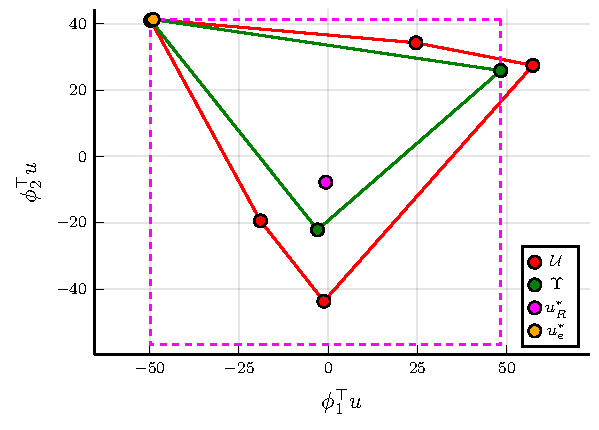
\includegraphics[scale=1.8]{../../pres_roil/plots/visual_solve_cheb.pdf}
                \end{center}
            \end{figure}
        \end{center}
    \end{block}

    \begin{block}{Regret Results}
        \begin{center}
            \begin{figure}
                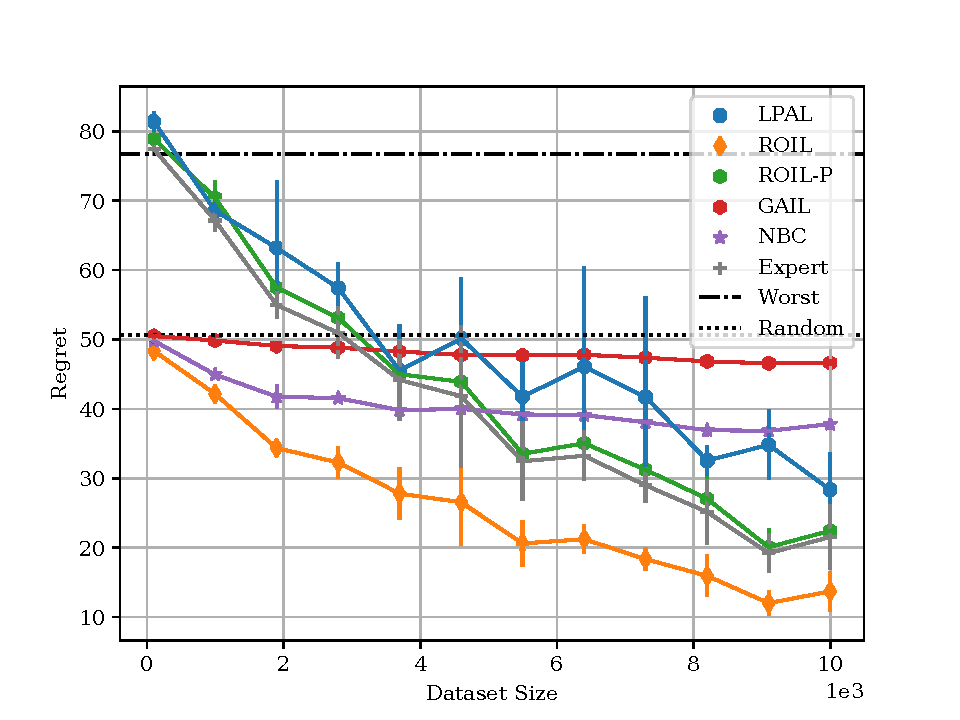
\includegraphics[scale=1.2]{../../pres_roil/plots/regrets/40x40_gridworld_on_policy_regret_regrets.pdf}
            \end{figure}
        \end{center}
    \end{block}
  \end{column}

% ===== COLUMN 3 ==========
  \begin{column}{0.3\linewidth}
    \begin{block}{Gridworld Results}
        \begin{center}
            \begin{figure}
                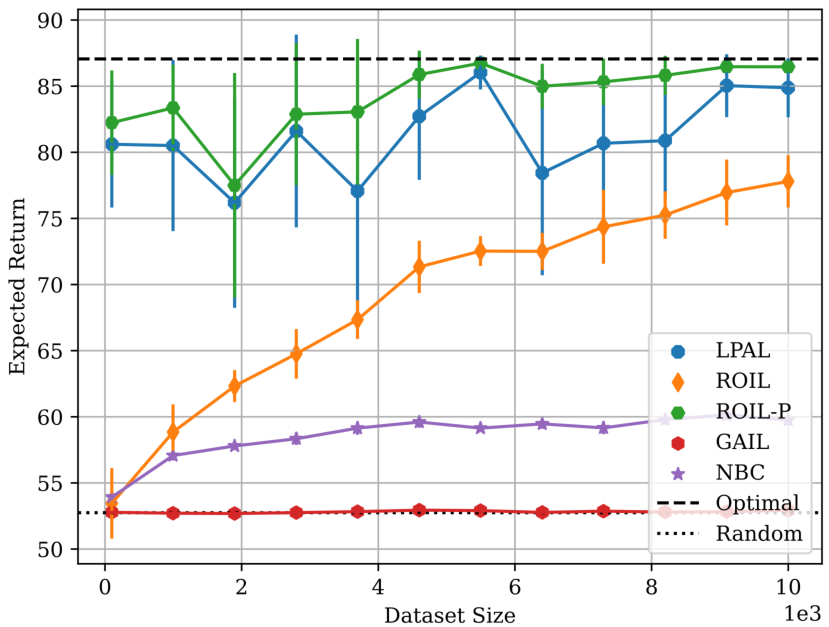
\includegraphics[scale=1.6]{../../pres_roil/plots/returns/40x40_gridworld_on_policy_returns_cropped.pdf}
                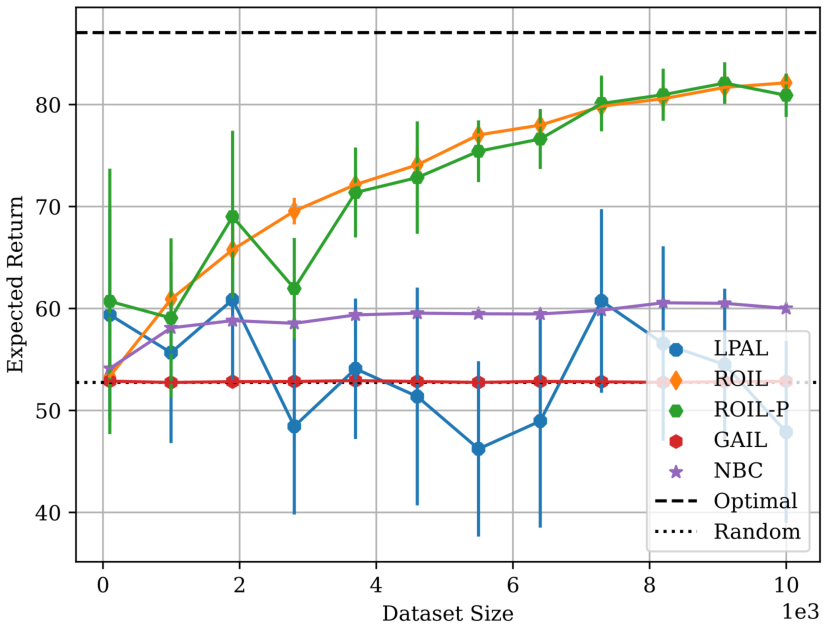
\includegraphics[scale=1.6]{../../pres_roil/plots/returns/40x40_gridworld_off_policy_returns_cropped.pdf}
            \end{figure}
        \end{center}
    \end{block}

    \begin{block}{Contact}
        \textbf{Gersi Doko}\\
        \textbf{Gersi.Doko@unh.edu}
    \end{block}
  \end{column}
\end{columns}
\end{frame}
\end{document}

%%% Local Variables:
%%% mode: latex
%%% TeX-master: t
%%% End:
